%!TEX root = ./report.tex
\section{Problem Analysis and Requirements}
\label{sec:problem_analysis_and_requirements}
In the following section we will analyse the problem, and discuss a set of requirements for a solution that is capable of editing a partial IFC model within a specific domain. This list should be thought of as a guideline for how one should ideally approach this problem.

\subsection{Problem Analysis}
\label{subsec:problem_analysis}
The separation of the construction and plumbing models makes it difficult to work on objects that are separated but interrelated. We focus on the case of IfcFlowSegments (i.e. a pipe), IfcWallStandardCases (a regular wall) and an IfcOpeningElement (an opening in a regular wall). Jørgensen mentions that a possible solution to the problem is to allow the building service engineer, responsible for the plumbing installations, to create a message with precise information about required openings for the pipes\,\cite{jorgensen12}. This message could then be handed to the construction engineer, so that he can verify that these are properly placed. As such, the primary goal of the solution is to enable the user to work on a subset of the IFC model involving pipes, openings, and walls. In Figure \ref{fig:ifcheirachy}, a graphical representation of this subset is presented.

\begin{figure}[t]
    \centering
        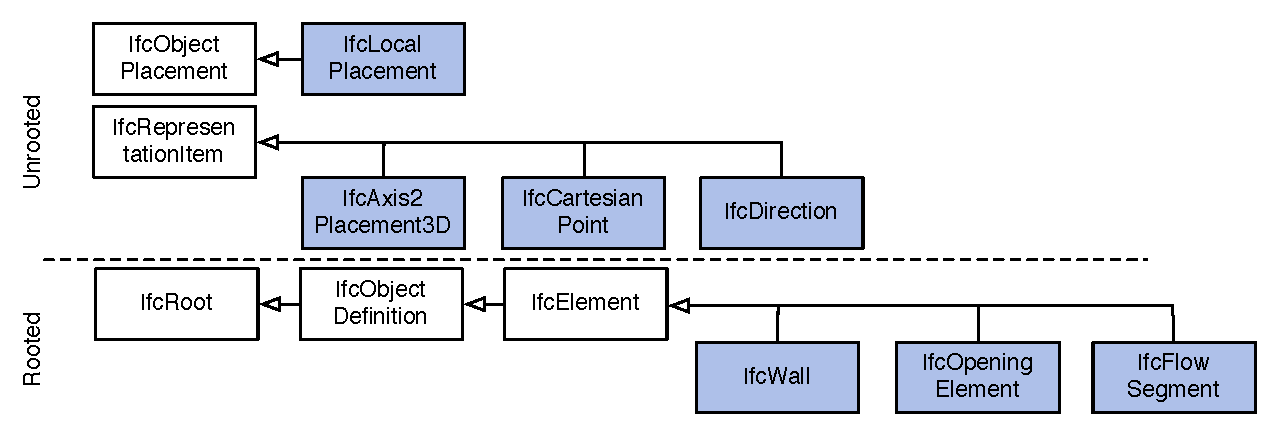
\includegraphics[width=110mm]{images/IfcHeirachy.pdf}
    \caption{A graphical representation of the subset used, excluding relational objects for the sake of simplicity. The concrete classes of the chosen subdomain are highlighted in blue.}
    \label{fig:ifcheirachy}
\end{figure}

\subsection{Requirements}
\label{subsec:requirements}
\subsubsection{R1. Working with a Partial Model}
With the aforementioned complexities and challenges of IFC in mind, a primary focus is to be able to extract a well-specified subset of an IFC model. It is desirable to have an architecture that separates the extraction of a partial model from the rest of the workflow. This component will only extract the IFC elements that we are interested in. This should make the component easier to reuse, and make it easier to verify that the extraction is performed correctly.

Furthermore, a clear domain definition is needed to implement and verify the extraction of the partial model. Achieving this in a concise but generic way is not trivial. An evolving standard for doing this is via Model View Definitions (MVD)\,\cite{nour08}, which allow fine-grained definitions of IFC subsets using XML. The non-profit organisation, buildingSMART, that supports open source BIM software, propagates MVD as their standard.\footnote{buildingSMART, MVD, \url{http://buildingsmart.com/standards/mvd}} Nour discusses this and other challenges when working with partial editing on IFC\,\cite{nour08}. Unfortunately, it was not possible to obtain the product of Nour's project. Even though MVD seems to be a promising approach for extracting IFC subsets, it is outside the scope of this project to develop this functionality ourselves. We found that simply defining a partial model with MVD is in itself a somewhat complex task. Therefore, for the purposes of designing a single experimental DSL with only a few IFC classes, we argue that a more informal definition of the domain is sufficient and will simplify the development process.

\subsubsection{R2. Correct Meta Model}
It is vital for the solution that the IFC meta model is in fact correct. This point may seem obvious at first, but in our experience, finding a correct EMF meta model that reflects the actual IFC standard is difficult. In particular, finding a meta model with a proper serialiser and deserialiser that converts from either IFC-EXPRESS or ifcXML to the corresponding Ecore instance can be difficult. Further, IFC models are not treated consistently across existing BIM software. Thus, one must be aware of inconsistencies\,\cite[p. 4]{quteprints37725}.

\subsubsection{R3. Valid Model Transformations}
An ideal solution would feature model transformations that are verifiable and correct. By verifiable, we mean being able to trace or test that transformations actually occur in the way that we expect. By correct, we mean not corrupting any model structure during a transformation. However, with the complexity of IFC in mind, we allow that some constraints are broken in the IFC model at the end of the transformation. A possible scenario is that in an IFC model, all pipe objects could be referenced by some central element, e.g. for calculation of maintenance costs for these. It would be difficult to require and assert that no such constraints are broken in the general case, and is a problem outside the scope of this project.

\subsubsection{R4. A Simple DSL}
The simple DSL will demonstrate that the editing of partial models is feasible for our own, as well as other, similar subdomains of IFC. The implementation will show how a small, but significant domain can be managed separately from the full IFC model. To support extensibility and reusability, it should be built with widely used tools, like the ones in EMF.  One could imagine that a future solution would have a visual syntax instead of a textual syntax.

\subsubsection{R5. Structural Editing}
It must be possible to use the DSL to add and remove elements. This is required to resemble a real-world scenario, where an element could be missing. The solution must be able to do this for flow segments and openings, without corrupting the IFC model. Structural editing of walls is not needed for the workflow described above, so it may be omitted.

\subsubsection{}
This concludes the list of desirable features, but please note that it is only a core selection, and that many extensions could be added to it. Some of these will be discussed in Section \ref{sec:plan_for_future_projects} as ideas for a future projects.

